\section{ 素直に言えなくて}
\large{

\ruby{星}{ほし}\ruby{降}{ふ}る\ruby{夜}{よる}は いつも Lonely-night

\ruby{溜}{た}め\ruby{息}{き}で \ruby{霞}{かす}んでる

\ruby{冷}{つめ}たい \ruby{ベッド}{bed}は \ruby{少}{すこ}し

\ruby{広}{ひろ}すぎて \ruby{眠}{ねむ}れない
\\

やさしすぎるから

つらくなってゆく

このまま ずっと \ruby{気付}{きづ}かないふりで

\ruby{笑顔}{えがお}に\ruby{変}{か}えたいの
\\

“ひとりにしないでね”って \ruby{素直}{すなお}に \ruby{言}{い}えなくて
\\

\parpic[r]{
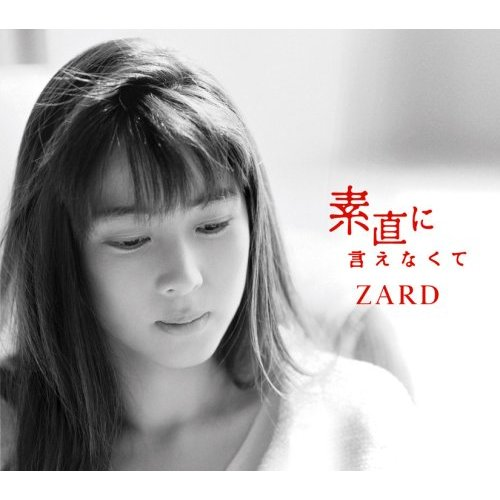
\includegraphics[width=0.4\textwidth]{S45.jpg}}

\ruby{腕}{うで}を\ruby{組}{く}んで \ruby{歩}{ある}いた Rainly-night

あたたかさに \ruby{酔}{よ}って

\ruby{夢}{ゆめ}を \ruby{見}{み}て いたいから

うしろは \ruby{振}{ふ}り\ruby{向}{む}かない
\\

\ruby{楽}{たの}しかったけど つらくなってゆく

これからは \ruby{強}{つよ}くなるから

きっと \ruby{涙}{なみだ}は \ruby{見}{み}せないわ
\\

“ひとりにしないでね”って \ruby{素直}{すなお}に \ruby{言}{い}えなくて
\\

やさしすぎるから つらくなってゆく

このまま ずっと \ruby{気付}{きづ}かないふりで

\ruby{笑顔}{えがお}に\ruby{変}{か}えたいの

“ひとりにしないでね”って \ruby{素直}{すなお}に \ruby{言}{い}えなくて

}